\documentclass[../Main.tex]{subfiles}

\begin{document}

\section{Experiment}
We now look at running the simulation, and analyzing the results. First, we look at some theoretical results pertaining to the four geometrical invariants under question - time reversibilty, total energy, total linear momentum, and total angular momentum. Then, we look at running the simulation for different values of the parameters $\beta$ and $\gamma$.
We will assume that the simulations have the following initial configuration (unless stated otherwise):

\begin{table}[H]
	\centering
	\begin{tabular}{ |l|r| }
		\hline
		Parameter & Initial Value \\
		\hline
		No. of particles & 864 \\
		Temperature & 1 K\textsuperscript{*} \\
		Density & $38.744 \mbox{ m}^{*}\sigma^{*^{-3}}$ \\
		h & 0.032 \\
		$N_{e}$ & 100 \\
		$N_{f}$ & 500 \\
		$N_{s}$ & 10 \\
		$N_{n}$ & 15 \\
		\hline
	\end{tabular}
	\caption{Initial Configuration for molecular simulations}
	\label{tbl:initial_configuration_simulation}
\end{table}

The last four elements in the table indicate that the simulation will initially be equilibrated for 100 iterations, and then run for 500 iterations where samples will be collected every 10 iterations (giving a total of 50 samples). The list of neighbours will be updated every 10 iterations in both the equilibration and final stages.

\subsection{Time Reversibility}
The molecular dynamics system is time reversible - if we go from state $s_{1}$ to state $s_{2}$ in time $\delta t$, then we can return to state $s_{1}$ from state $s_{2}$ in time $\delta t$ by reversing the signs on the velocities. This can be seen formally by applying the transformation $t \mapsto -t$ to Equation~\ref{eqn:mol_hamiltonian_separate} - the position $q$ does not change, but the sign on momentum $p$ gets reversed.
\begin{align*}
q \mapsto q = \tilde{q},  \quad \quad p \mapsto -p = \tilde{p}.
\end{align*}
Then
\begin{alignat*}{4}
	\dot{\tilde{q}} &= \frac{d\tilde{q}}{d\left(-t\right)} \quad &&= -\nabla_{\tilde{p}}H \quad &&= \nabla_{p}H \quad &&= \dot{q},\\
	\dot{\tilde{p}} &= \frac{d\tilde{p}}{d\left(-t\right)} \quad &&= -\nabla_{\tilde{q}}H \quad && =-\nabla_{q}H \quad &&= \dot{p}.
\end{alignat*}
Thus, the Hamiltonian system is time reversible.

We say that a numerical one-step method $\Phi_{h}: (\vec{x}_{i},\vec{v}_{i}) \mapsto (\vec{x}_{i+1},\vec{v}_{i+1})$ is time reversible if $\Phi_{h} = \Phi_{-h}^{-1}$. Informally, this means that if we exchange $i \leftrightarrow i+1$ and replace $h$ by $-h$ in our origina method, then we should get the same method back.
In order to ascertain which Newmark Beta methods are reversible, we cite \cite{Paganini2017}:
\begin{theorem}The maximal order of a reversible one-step method is always even. \label{thm:reversible_even_order} \end{theorem}
 As Newmark Beta methods have maximal order 2 only if $\gamma = \frac{1}{2}$, the contrapositive of \ref{thm:reversible_even_order} states that any scheme with $\gamma \neq \frac{1}{2}$ is not reversible. Now, we claim
\begin{claim} Any Newmark Beta method with $\gamma = \frac{1}{2}$  is reversible. \end{claim}
\begin{proof}
A Newmark Beta scheme with $\gamma = \frac{1}{2}$ has the form
\begin{align}
		\vec{v}_{i+1} & = \vec{v}_{i} + h\left(\frac{1}{2}\vec{a}_{i} + \frac{1}{2}\vec{a}_{i+1}\right), \label{eqn:target_reversible_newmark-beta_v}\\
		\vec{x}_{i+1} & = \vec{x}_{i} + h\vec{v}_{i} + \frac{h^2}{2}\left[(1-2\beta)\vec{a}_{i} + 2\beta\vec{a}_{i+1}\right].  \label{eqn:target_reversible_newmark-beta_x} 
\end{align}
Swapping $i \leftrightarrow i+1$ and replacing $h$ with $-h$
\begin{align}
		\vec{v}_{i} & = \vec{v}_{i+1} - h\left(\frac{1}{2}\vec{a}_{i+1} + \frac{1}{2}\vec{a}_{i}\right),  \label{eqn:current_reversible_newmark-beta_v}\\
		\vec{x}_{i} & = \vec{x}_{i+1} - h\vec{v}_{i+1} + \frac{h^2}{2}\left[(1-2\beta)\vec{a}_{i+1} + 2\beta\vec{a}_{i}\right]. \label{eqn:current_reversible_newmark-beta_x} 
\end{align}
It is straight-forward to see that Equation~\ref{eqn:current_reversible_newmark-beta_v} is the same as Equation~\ref{eqn:target_reversible_newmark-beta_v}.
For Equation~\ref{eqn:current_reversible_newmark-beta_x}, we see
\begin{align*}
	\vec{x}_{i+1} & = \vec{x}_{i} + h\vec{v}_{i+1} - \frac{h^2}{2}\left[(1-2\beta)\vec{a}_{i+1} + 2\beta\vec{a}_{i}\right] \\
	& = \vec{x}_{i} + h\left(\vec{v}_{i} + \frac{h}{2}\vec{a}_{i} + \frac{h}{2}\vec{a}_{i+1}\right) - \frac{h^2}{2}\left[(1-2\beta)\vec{a}_{i+1} + 2\beta\vec{a}_{i}\right] \\
	& = \vec{x}_{i} + h\vec{v}_{i} + \frac{h^2}{2}\left[\left(1-2\beta\right)\vec{a}_{i} + 2\beta\vec{a}_{i+1}\right].
\end{align*} 
\end{proof} 
 
While the schemes may be time reversible in theory, the rounding-off errors in practice mean that we may not get back the initial state of the system after reversing the velocities. We test this for different values of $\beta$ and $\gamma$ over different. In these experiments, we do not differentiate between equilibration and final iterations, and reverse the sign on the velocities after half of the total number of iterations have been completed. 

We can see in Figure~\ref{fig:time_reversible_b0.00g0.50_1000} that errors are introduced while reversing 500 iterations of the Velocity Verlet algorithm. While the particles are almost at their initial positions, the velocities tend to be higher than those in the initial state. This is worsened when we reverse 500 steps of the Newmark Beta method with $\beta = 0$ and $\gamma = 0.75$. As noted earlier, this is not a reversible method and we can see that in Figure~\ref{fig:time_reversible_b0.00g0.75_1000}, where the velocity histogram is much narrower that it should be. Figure~\ref{fig:time_reversible_b0.00g0.75_1000,50} is interesting - the method clearly does not conserve the total energy in the system if it is reversed after 500 iterations (samples have been taken every 5 iterations). However, if the reversal happens after a short period of time (25 iterations) then we get that the total energy of the system is reversed as well. Figure~\ref{fig:time_reversible_b0.25g0.50_250} shows the errors in time reversibility for an implicit method wtih $\beta = 0.25$ and $\gamma = 0.5$ (which is time reversible). The histograms seem to agree very well, but if we take the absolute error in velocities of each point, we get that the mean absolute error is 0.233 with a standard deviation of 0.174 - which is considerably large given that velocities range over $\left[-0.6, 0.6\right]$. In comparison, the Velocity Verlet method has a mean absolute error of 0.158 with a standard deviation of 0.118.

\begin{figure}[H]
\centering
 	\begin{tabular}{@{}cc@{}}
		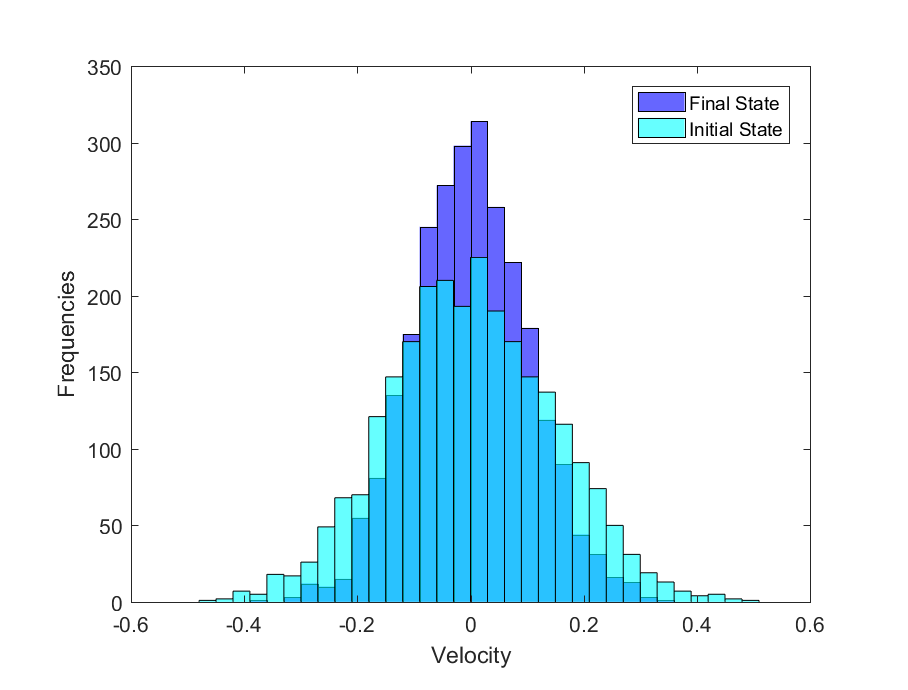
\includegraphics[width=0.5\textwidth]{time_reversible_b0,0g0,50_1000_velocity_histogram.eps} &
    		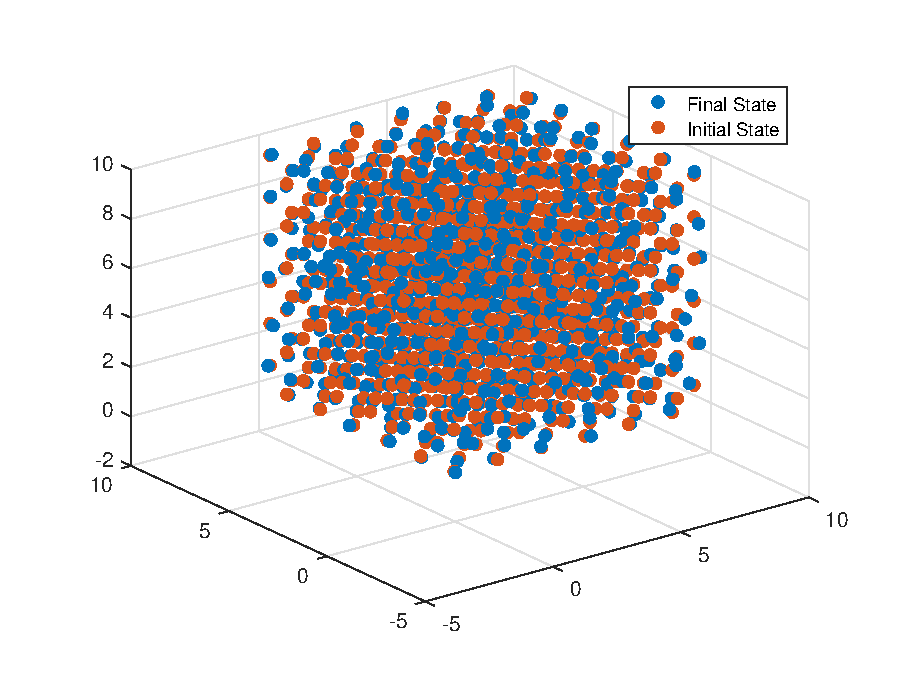
\includegraphics[width=0.5\textwidth]{time_reversible_b0,0g0,50_1000_position_overlay.eps} \\
	\end{tabular}
  	\caption{Changes in position and velocities for $\beta = 0.00$ and $\gamma = 0.50$ after reversing 500 steps}
	\label{fig:time_reversible_b0.00g0.50_1000}
\end{figure}

\begin{figure}[H]
\centering
 	\begin{tabular}{@{}cc@{}}
		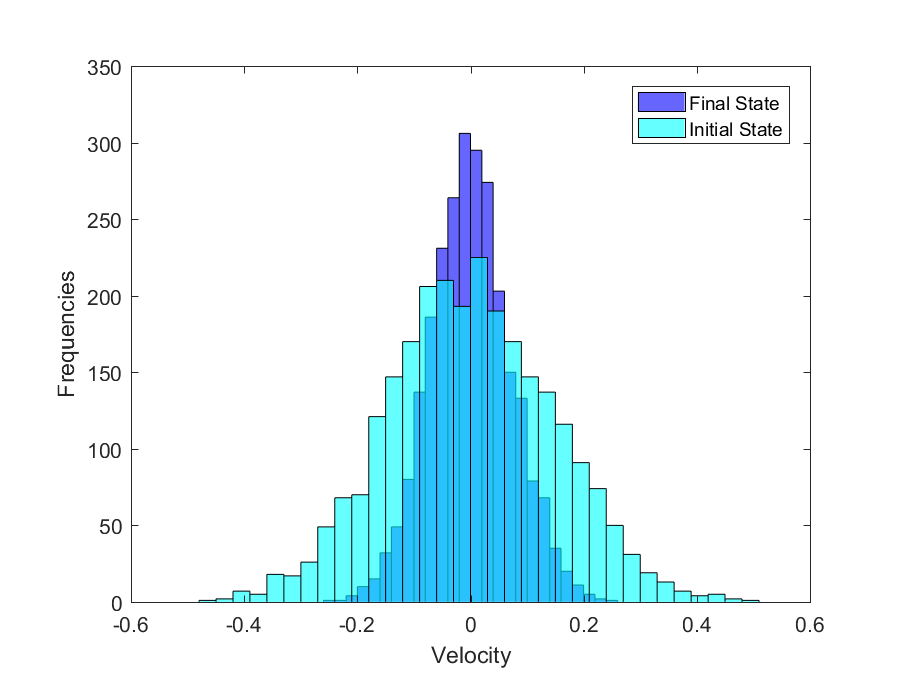
\includegraphics[width=0.5\textwidth]{time_reversible_b0,0g0,75_1000_velocity_histogram.eps} &
    		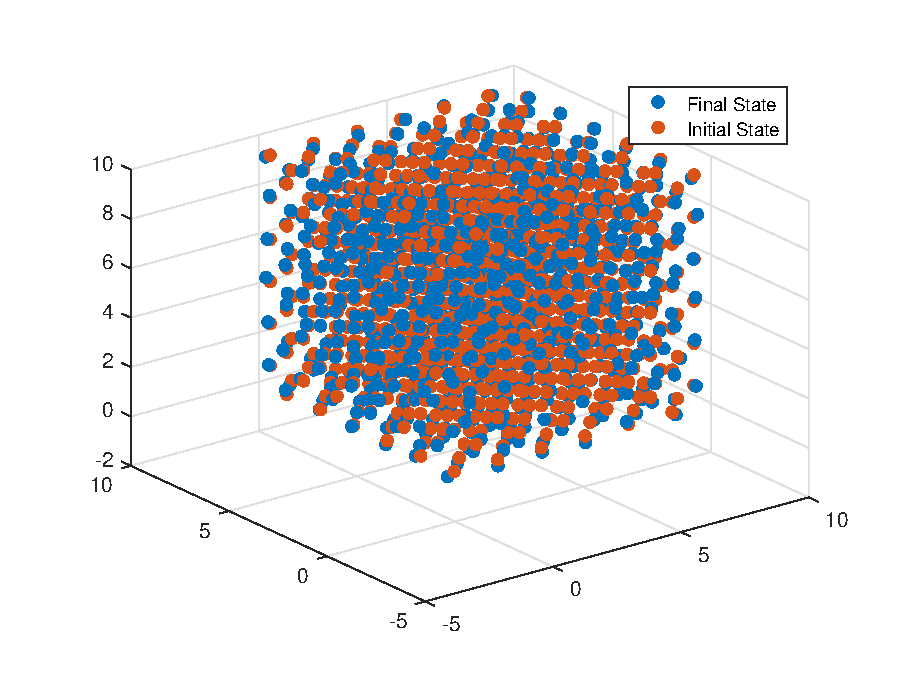
\includegraphics[width=0.5\textwidth]{time_reversible_b0,0g0,75_1000_position_overlay.eps} \\
	\end{tabular}
  	\caption{Changes in position and velocities for $\beta = 0.00$ and $\gamma = 0.75$ after reversing 500 steps}
	\label{fig:time_reversible_b0.00g0.75_1000}
\end{figure}

\begin{figure}[H]
\centering
 	\begin{tabular}{@{}cc@{}}
    		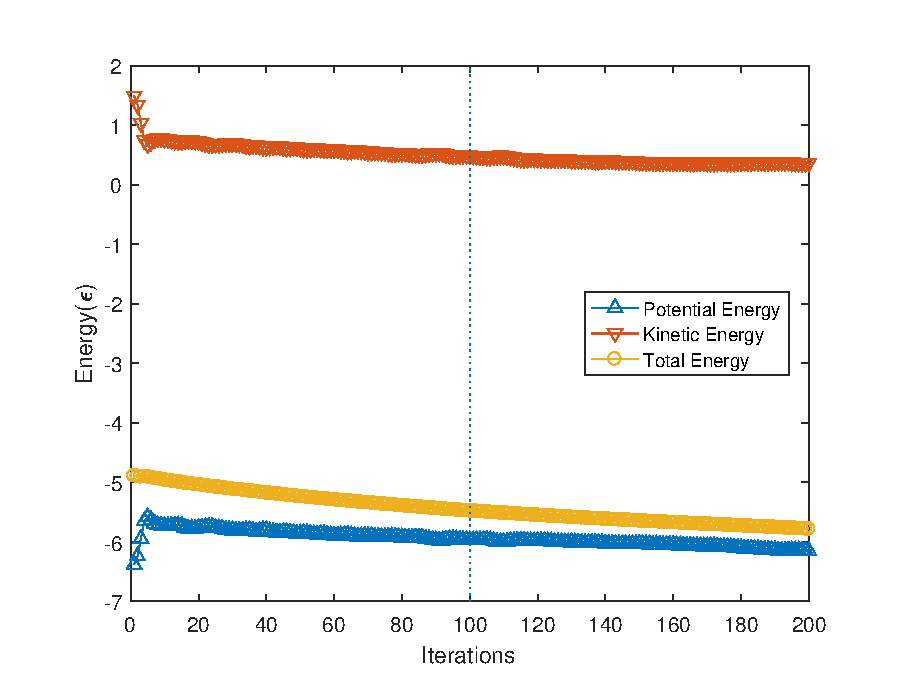
\includegraphics[width=0.5\textwidth]{time_reversible_b0,0g0,75_1000_energy.eps} &
    		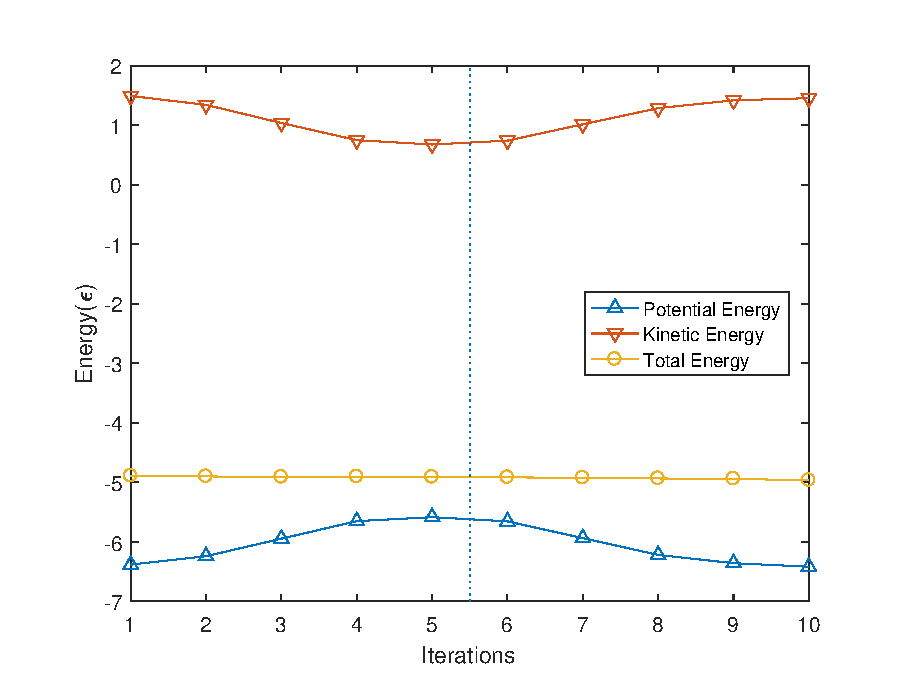
\includegraphics[width=0.5\textwidth]{time_reversible_b0,0g0,75_50_energy.eps} \\
	\end{tabular}
  	\caption{Difference in behaviour of total  energy for $\beta = 0.00$ and $\gamma = 0.75$ over different timesteps}
	\label{fig:time_reversible_b0.00g0.75_1000,50}
\end{figure}

\begin{figure}[H]
\centering
 	\begin{tabular}{@{}cc@{}}
    		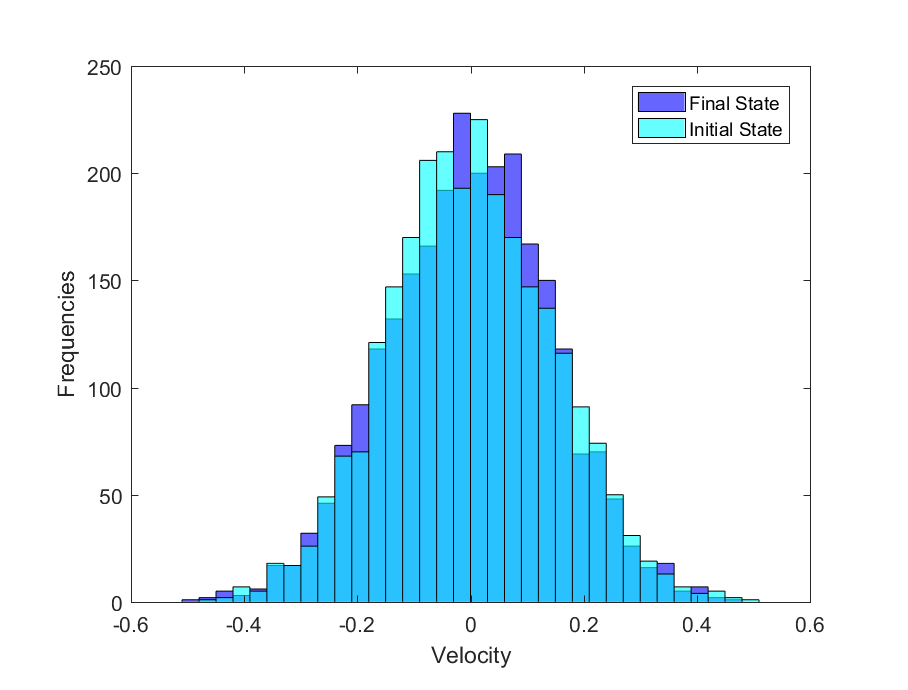
\includegraphics[width=0.5\textwidth]{time_reversible_b0,25g0,50_250_velocity_histogram.eps} &
    		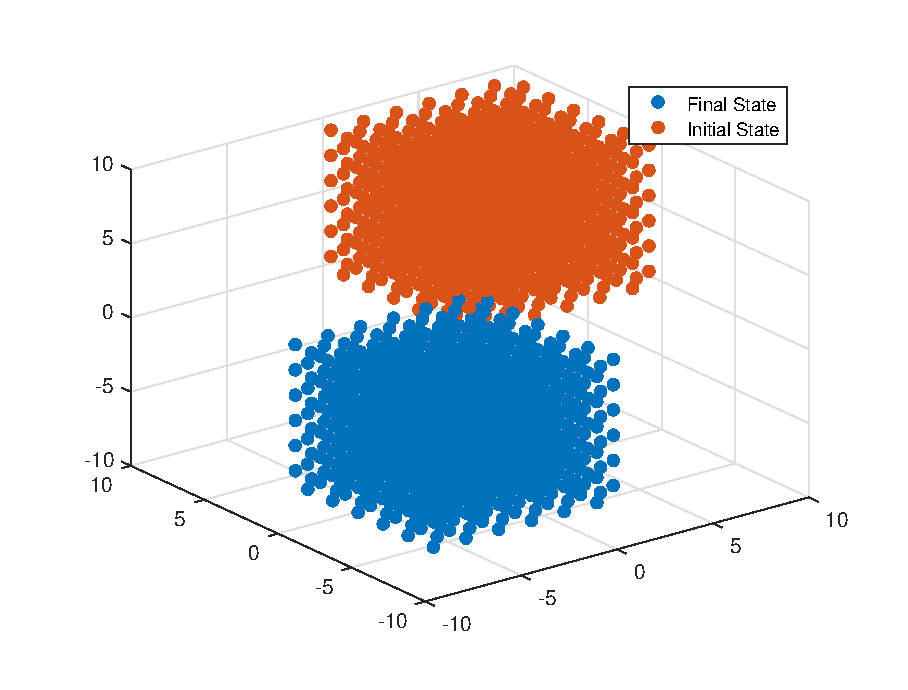
\includegraphics[width=0.5\textwidth]{time_reversible_b0,25g0,50_250_position_overlay.eps} \\
	\end{tabular}
  	\caption{Changes in position and velocities for $\beta = 0.25$ and $\gamma = 0.50$ after reversing 125 steps}
	\label{fig:time_reversible_b0.25g0.50_250}
\end{figure}
 The coordinates do not seem to be conserved, but rather translated. A possible reason for this is that in the Newton-Raphson Iteration, we introduce a small noise to  $\vec{x}_{i}$ before calculating $\vec{x}_{i+1}$, to prevent the Jacobian from being sparse. This seems to be a plausible reason, as all the coordinates have a pointwise absolute error of 1.600 (accurate to three decimal places).

\subsection*{Aside: First Integrals}
The next three invariants - total energy, linear momentum, and angular momentum - follow readily from Newton's Laws of Motion as there is no external force on the system. In order to simplify checking which methods preserve these invariants the best, we introduce the concept of first integrals. \\
A non-constant function $I(y)$ is a \textit{first integral} (or invariant) of the differential equation $\dot{y} = F(y)$ if $I(y(t))$ is constant along every solution, or equivalently, if
\begin{align}
\nabla I(y)F(y) = 0    \quad \quad \quad  \forall y. \quad \cite{HarierLubichWanner2003} \label{eqn:grad_first_integral_zero}
\end{align}
Total energy, total linear momentum, and total angular momentum are all first integrals \cite{HarierLubichWanner2003}. We look at proving this in the next subsections, adapting the proofs from \cite{HarierLubichWanner2003}.

\subsection{Total Linear Momentum}
 
\begin{theorem} Total linear momentum $P = \sum_{i=1}^{N} p_{i}$ is a first integral. \end{theorem}
\begin{proof}
\begin{align*}
\nabla P & = \frac{dP}{dt} = \sum_{i=1}^{N} \frac{dp_{i}}{dt} \\
&=\sum_{i=1}^{N}\sum_{j=1}^{N}\nu_{ij}\left(q_{i} - q_{j}\right) \\
& = 0 \qquad \qquad \qquad \qquad \cdots \mbox{ as }\nu_{ij} = \nu_{ji} \forall i, j
\end{align*}
\end{proof} 

Total linear momentum - as the name suggests - is a linear first integral. Most numerical methods preserve linear first integrals - in fact, it is a property shared by all Runge-Kutta methods. Indeed, this holds true for the entire family of Newmark Beta methods as well.
\begin{claim} All Newmark Beta methods preserve linear first integrals \end{claim}
\begin{proof}
Let $I(\vec{x}, \vec{v}) = b^{T}\vec{x} + c^{T}\vec{v}$ be a linear first integral, where $b$ and $c$ are some constant vectors.
By the defintion of first integrals, we want that $I'(\vec{x}, \vec{v})= 0$ for all $\vec{x}, \vec{v}$.
But $I'(\vec{x}, \vec{v}) = b^{T}\vec{v} + c^{T}\vec{a(\vec{x})}\ = 0$, implying that $b^{T} = 0$ and $c^{T}\vec{a}(\vec{x}) = 0$ for all $\vec{x}$. So, $I(\vec{x}, \vec{v}) = I(\vec{v}) = c^{T}\vec{v}$ (This makes sense in a real-world scenario as total linear momentum depends only on the velocity of the body, and not its position).\\
Now, we multiply $c^{T}$ to the velocity portion of the Newmark Beta method and get that
\begin{align*}
I\left(\vec{v}_{i+1}\right) &= c^{T}\vec{v}_{i+1} \\
&= c^{T}\vec{v}_{i} + h\left[\left(1-\gamma\right)c^{T}\vec{a}(\vec{x}_{i}) + \gamma c^{T}\vec{a}(\vec{x}_{i+1})\right] \\
&= c^{T}\vec{v}_{i} = I\left(\vec{v}_{i}\right)
\end{align*} 
\end{proof}

As we calibrated the system to have an initial total linear momentum of zero, the total linear momentum will be zero for all of the trials. As this holds true for all members of the Newmar Beta family, we do not present experimental results for this property, but rather state that in all trials, the total linear momentum was almost zero - it cannot be exactly zero due to inaccuracies introduced by floating-point arithmetic and rounding-off, but these errors were in the range of $10^{-10}$.

\subsection{Total Angular Momentum}

\begin{theorem} Total angular momentum $L = \sum_{i=1}^{N} q_{i} \times p_{i}$ is a first integral. \end{theorem}
\begin{proof}
\begin{align*}
\nabla L & = \sum_{i=1}^{N} \frac{d}{dt} \left(q_{i} \times p_{i}\right) \\
& = \sum_{i=1}^{N} \left(\dot{q}_{i} \times p_{i} + {q}_{i} \times \dot{p}_{i}\right) \\  
& = \sum_{i=1}^{N} \left( \frac{1}{m_{i}}p_{i} \times p_{i} + q_{i} \times \sum_{j=1}^{N}\nu_{ij}\left(q_{i} - q_{j}\right)\right) \\  
& = \sum_{i=1}^{N} \left( \frac{1}{m_{i}}p_{i} \times p_{i}\right) +  \sum_{i=1}^{N}\sum_{j=1}^{N} \left(q_{i} \times \nu_{ij}\left(q_{i} - q_{j}\right)\right) \\
& = 0  \qquad \qquad \qquad \qquad \cdots \mbox{ as }\nu_{ij} = \nu_{ji} \mbox{ and } p_{i} \times p_{i} = 0 \,\forall i, j
\end{align*}
\end{proof}

Total angular momentum is a quadratic first integral. By Noether's Theorem, it has the form $I(\vec{x}, \vec{v}) = \vec{v}^{T}\left(C\vec{x} + d\right)$, where $C$ is a constant square matrix and $d$ is a constant vector \cite{HarierLubichWanner2003}.
We have the Velocity Verlet method preserves quadratic integrals of this form, and hence, total angular momentum. To see this, we need to express it as the composition of two half-step methods:
\begin{align}
	\begin{split}
		\vec{v}_{i+\frac{1}{2}} = \vec{v}_{i} + \frac{h}{2}\vec{a}(\vec{x}_{i}) \\
		\vec{x}_{i+\frac{1}{2}} = \vec{x}_{i} + \frac{h}{2}\vec{v}_{i+\frac{1}{2}}
	\end{split}
\end{align}
and
\begin{align}
	\begin{split}
		\vec{x}_{i+1} = \vec{x}_{i+ \frac{1}{2}} + \frac{h}{2}\vec{v}_{i+\frac{1}{2}} \\
		\vec{v}_{i+1} = \vec{v}_{i+\frac{1}{2}} + \frac{h}{2}\vec{a}(\vec{x}_{i+1})
	\end{split} \label{velocity_verlet_split_2}
\end{align}

\begin{theorem} The Velocity Verlet algorithm preserves quadratic first integrals of the form $I(\vec{x}, \vec{v}) = \vec{v}^{T}\left(C\vec{x} + d\right)$ \end{theorem}
\begin{proof}
We have that $I'(\vec{x}, \vec{v}) = \vec{a}(\vec{x})^{T}\left(C\vec{x} + d\right) + \vec{v}^{T}C\vec{v} = 0$ for all $\vec{x}, \vec{v}$.
Now,
\begin{align*}
\vec{v}_{i+\frac{1}{2}}^{T}\left(C\vec{x}_{i+\frac{1}{2}} + d\right) &= \vec{v}_{i+\frac{1}{2}}^{T}\left(C\vec{x}_{i} + \frac{h}{2}C\vec{v}_{i+\frac{1}{2}} + d\right) \\
&= \vec{v}_{i+\frac{1}{2}}^{T}\left(C\vec{x}_{i} + d\right) + \frac{h}{2}\vec{v}_{i+\frac{1}{2}}^{T}C\vec{v}_{i+\frac{1}{2}} \\
&= \left(\vec{v}_{i} + \frac{h}{2}\vec{a}(\vec{x}_{i})\right)^{T}\left(C\vec{x}_{i} + d\right)+ \frac{h}{2}\vec{v}_{i+\frac{1}{2}}^{T}C\vec{v}_{i+\frac{1}{2}} \\
&=\vec{v}_{i}^{T}(C\vec{x}_{i} + d) + \frac{h}{2}\left( \vec{a}(\vec{x}_{i})^{T}(C\vec{x}_{i} + d) + \vec{v}_{i+\frac{1}{2}}^{T}C\vec{v}_{i+\frac{1}{2}}\right) \\
&=\vec{v}_{i}^{T}(C\vec{x}_{i} + d) + I'(\vec{x}_{i}, \vec{v}_{i+\frac{1}{2}}) \\
&=\vec{v}_{i}^{T}(C\vec{x}_{i} + d)
\end{align*}

Similarly, we get from Equation~\ref{velocity_verlet_split_2} that
\begin{align*}
I(\vec{x}_{i+1}, \vec{v}_{i+1}) &=\vec{v}_{i+1}^{T}(C\vec{x}_{i+1} + d) \\
&= \vec{v}_{i+\frac{1}{2}}^{T}\left(C\vec{x}_{i+\frac{1}{2}} + d\right) \\
&=\vec{v}_{i}^{T}(C\vec{x}_{i} + d) \\
&= I(\vec{x}_{i}, \vec{v}_{i})
\end{align*}
\end{proof}

There are no other Newmark Beta methods that conserve total angular momentum \cite{Newmark1959}. To see this, we calculate
the difference between the angular momentum at time $t_{i+1}, L_{i+1}$ and time $t_{i}, L_{i}$ \cite{SimoTarnowWong1992}. We use the notation $\left(\vec{b}_{i}\right)_{k}$ to denote the $k^{th}$ entry of vector $\vec{b}$ at time $i$.
\begin{align*}
L_{i+1} -  L_{i} = \sum_{k=1}^{N}\left(q_{i+1}\right)_{k} \times \left(p_{i+1}\right)_{k} - \sum_{k=1}^{N}\left(q_{i}\right)_{k} \times \left(p_{i}\right)_{k}.
\end{align*}
Substituting in the Newmark Beta expressions for position and momentum, we get that
\begin{align}
L_{i+1} -  L_{i} = h^{2}\left(\gamma - \frac{1}{2}\right)\sum_{k=1}^{N} (\vec{a}_{i})_{k} \times (\vec{p}_{i})_{k} + h^{2}\beta\sum_{k=1}^{N} (\vec{a}_{i+1})_{k} \times (\vec{p}_{i+1})_{k} - (\vec{a}_{i})_{k} \times (\vec{p}_{i})_{k} . \label{eqn:angular_momentum_diff_identity}
\end{align}

Thus, we get that Equation~\ref{eqn:angular_momentum_diff_identity} is 0 only if $\beta = 0$ and $\gamma = \frac{1}{2}$. 
We can test this result in our experimental setup, varying the parameters $\beta$ and $\gamma$ to see which methods come close to preserving total angular momentum. Surprsingly, we get that the angular momentum is not experimentally preserved by the Velocity Verlet algorithm! Table~\ref{tbl:total_angular_momentum_50_iterations} shows the first five samples of total angular momentum taken during the simulation, depicting that the lack of clear trend in change of angular momentum. 
\begin{table}[h]
	\centering
	\begin{tabular}{ |r|r|r|r| }
		\hline
		Iteration & x-component & y-component & z-component\\
		\hline
		10 & 493.28 & -402.32 & 1407.30 \\
		20 & -4.80 & -10.18 & 914.24 \\
		30 & 320.20 & -147.35 & 980.93 \\
		40 & 717.70 & -181.21 & 704.27 \\
		50 & 594.66 & 152.47 & 507.19 \\
		\hline
	\end{tabular}
	\caption{Total angular momentum of the system over the first 50 iterations}
	\label{tbl:total_angular_momentum_50_iterations}
\end{table}

The reason behind this incoherent behaviour is the application of periodic boundary conditions. Angular momentum is defined relative to the origin as it is the cross product of position and momentum. When a particle moves out of the box, it reenters the box from the opposite face due to periodic boundary conditions - this creates a discontinuity in the position of the particle, and hence, a discontinuity in the the angular momentum of the particle. Note however, that the velocity of the particle does not change, and hence, linear momentum is preserved. We say that periodic boundary conditions preserve translational symmetry, but not rotational symmetry.
As a result, we have that in the simulations, no method will preserve total angular momentum. However, this will not affect the simulation as no thermodynamic property depends upon the angular momenta of the particles.
 
\subsection{Total Energy}

\begin{theorem} The total energy, or the Hamiltonian, is a first integral. \end{theorem}
\begin{proof}
From definitions,
$$
	\nabla H = \left(\nabla_{p}H^{T}, \nabla_{q}H^{T}\right)
$$
and
$$
	\frac{dH}{dt} =
		\begin{pmatrix*}[r]
			-\nabla_{q}H \\
			\nabla_{p}H
		\end{pmatrix*}
$$
Then, 
$$
\nabla H(p, q) \cdot \frac{dH}{dt} = \nabla_{p}H^{T}\cdot-\nabla_{q}H + \nabla_{q}H^{T}\cdot \nabla_{p}H = 0
$$ 
\end{proof} 

The case of total energy is more complicated than those of the other geometric invariants. As we will see later, it is not the Hamiltonian is not preserved by some methods, but rather it is the `shadow' variant of the Hamiltonian.

We start by quoting Simo, Tarnow, and Wong from \cite{SimoTarnowWong1992}:
``\textit{What may seem surprising is that all of the implicit members of the Newmark family, perhaps the most widely used time-stepping algorithms in nonlinear structural dynamics, are not designed to conserve energy and also fail to conserve momentum. Among the explicit members, only the central difference method preserves momentum.}''	

Here, the ``central difference method'' refers to the Velocity Verlet Scheme, i.e., $\beta = 0$ and $\gamma = \frac{1}{2}$. But what is so significant about $\gamma = \frac{1}{2}$ that it appears everywhere? The answer lies in the interpretation of $\gamma$ in the Newmark Beta equations: $\gamma$ controls the damping in system by a factor of $\gamma - \frac{1}{2}$. So, if $\gamma > \frac{1}{2}$, then the energy in the system is damped, and if $\gamma < \frac{1}{2}$, the energy in the system grows. We see this numerically in Figure~\ref{fig:energy_time_series_damping}. 
\begin{figure}[H]
\centering
 	\begin{tabular}{@{}cc@{}}
		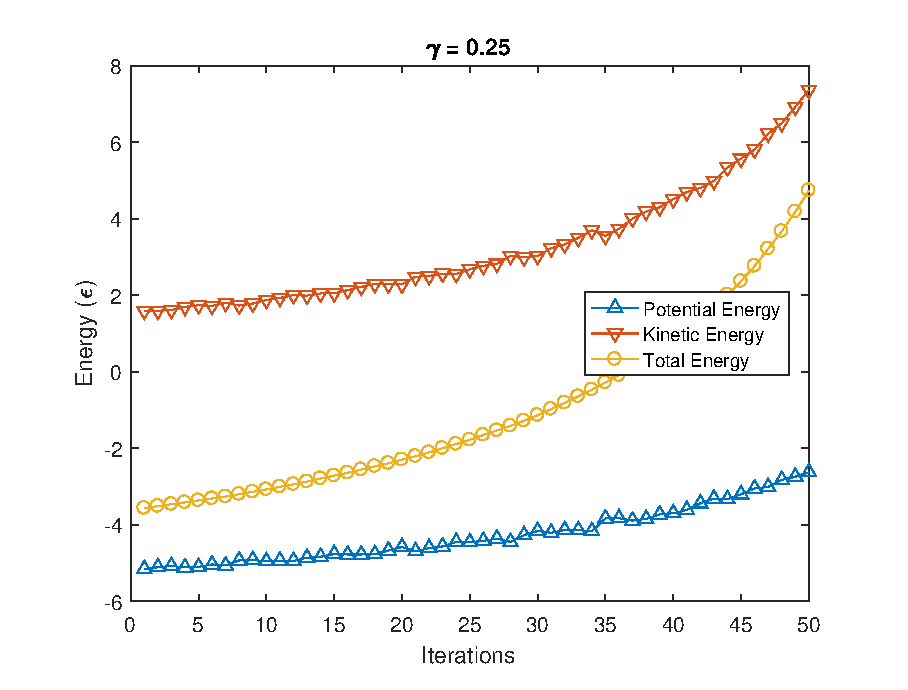
\includegraphics[width=0.5\textwidth]{energy_b0,00_g0,25.eps} &
    		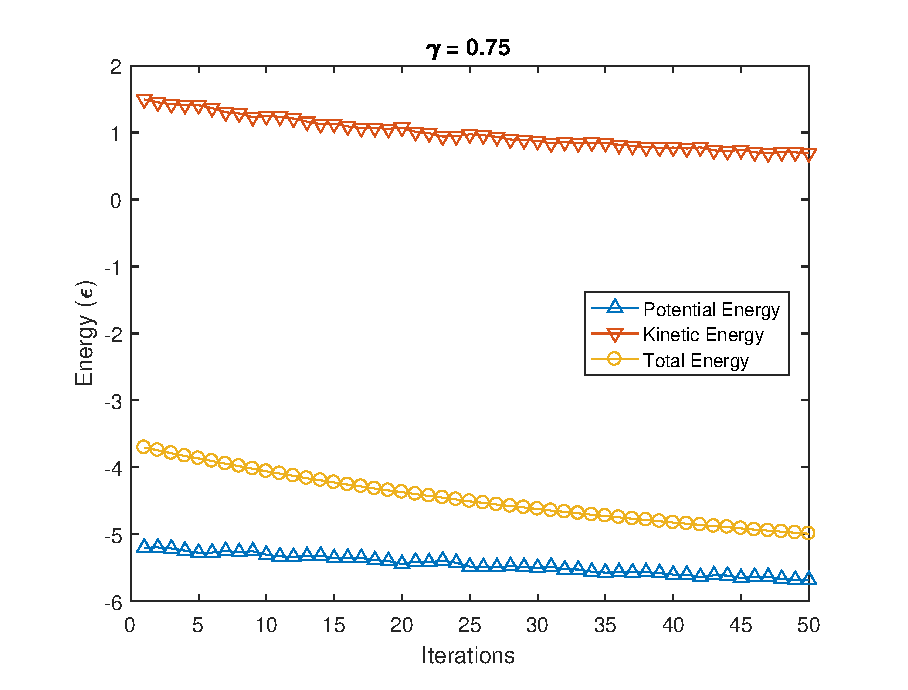
\includegraphics[width=0.5\textwidth]{energy_b0,00_g0,75.eps} \\
	\end{tabular}
  	\caption{Energy time series for two explicit Newmark Beta methods}
	\label{fig:energy_time_series_damping}
\end{figure}

Thus, we will restrict our numerical investigation to the cases where $\gamma = \frac{1}{2}$ and $\beta \in \left[0, \frac{1}{2}\right]$.
For the explicit case ($\beta = 0$), we will use the initial conditions as defined in Table~\ref{tbl:initial_configuration_simulation}. For the implicit cases, however, we set $N_{e} = 50$ and $N_{f} = 200$ ($N_{n}$ and $N_{s}$ remain unchanged). Understandably, this could hamper the simulation; however, an implicit Newmark Beta method takes an average of 1100 s to perform 250 overall iterations, as compared to an explicit Newmark Beta method that takes an average of 170 s to perform 600 iterations. This slow speed of execution makes it impossible to run longer simulations for different parameters multiple times.

The results of the investigation are visible in Figures~\ref{fig:energy_time_series_velocity_verlet} and \ref{fig:energy_time_series_gamma_0,50_implicit_beta}. We can see that the Velocity Verlet algorithm - ever dependable, as always - shows minimal change in the energy of the system over 500 iterations. The reason for this behaviour is that the Velocity Verlet shows a property known a symplecticity. A discussion on what is symplecticity, and what does it entail is beyond the scope of this project. However, the keen reader is can find a detailed, yet approachable, discussion in \cite{Sanz-serna1992}. As the solutions of a Hamiltonian system are also symplectic, we have that the Velocity Verlet is performs well as a numerical approximation scheme due to its symplecticity. Nonetheless, we can see that the total energy is not constant throughout the run - it decreases from $-3.36\varepsilon$ and $-3.79\varepsilon$. This gives us that the Velocity Verlet algorithm does not preserve the energy of the system (energy is not constant throughout the simulation), but rather conserved. We quote \cite{Harier2006}
\begin{theorem}
For a Hamiltonian $H(p, q)$, the total energy of a numerical solution $\left(p_{n}, q_{n}\right)$ of the Velocity Verlet method satisfies 
$\left|H\left(p_{n}, q_{n}\right) - H\left(p_{0}, q_{0}\right) \right| \leq Ch^{2}$, where $C$ is a constant independent of $h$.
\end{theorem}

\begin{figure}[H]
\centering
 	\begin{tabular}{@{}cc@{}}
		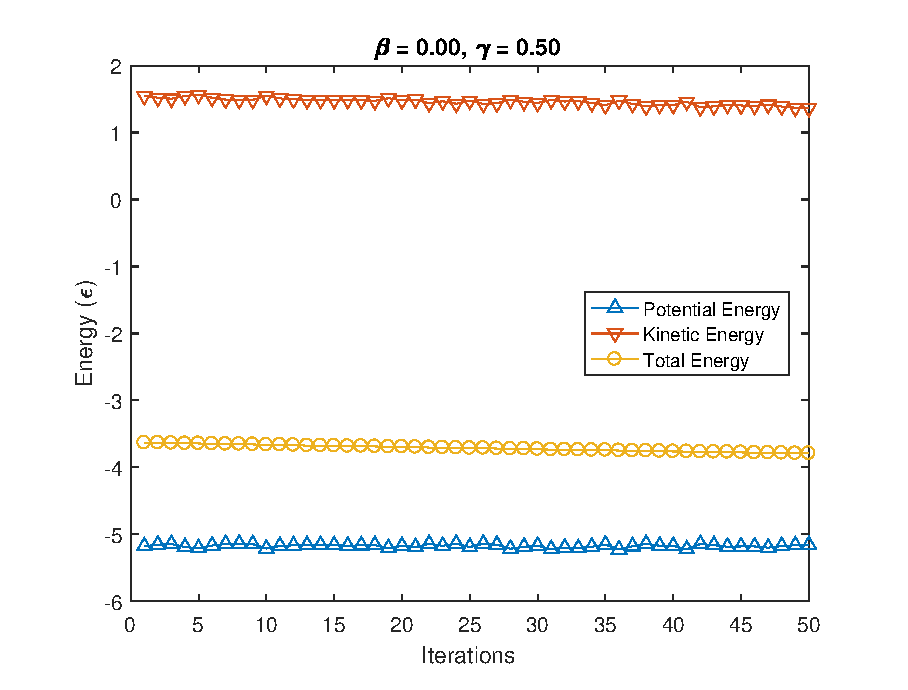
\includegraphics[width=0.5\textwidth]{energy_b0,00_g0,50.eps}
		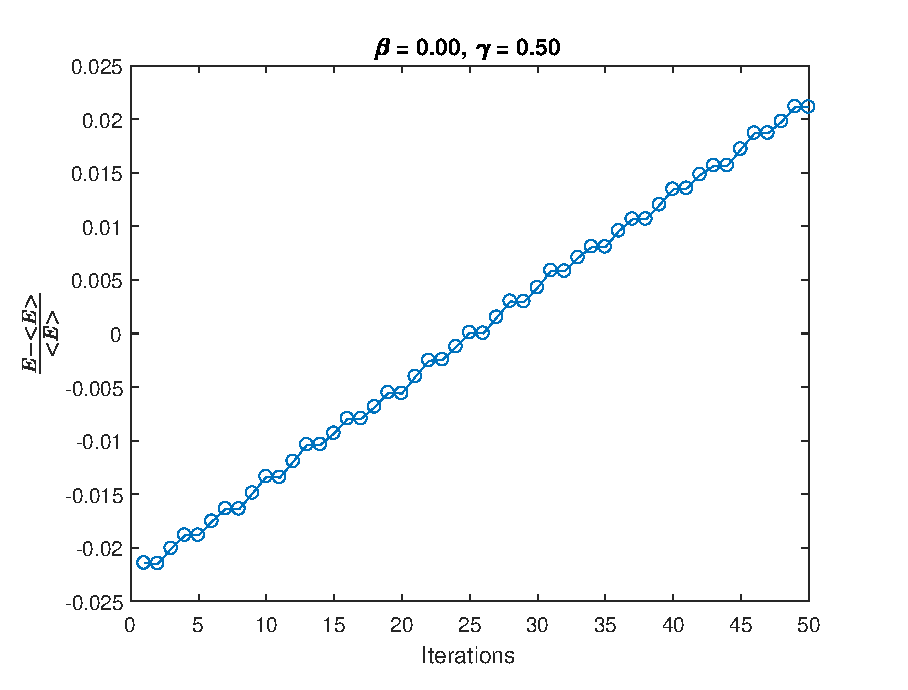
\includegraphics[width=0.5\textwidth]{energy_b0,00_g0,50_fluctuation.eps}
	\end{tabular}
	\caption{Energy time series for Velocity Verlet method}
	\label{fig:energy_time_series_velocity_verlet}
\end{figure}

\begin{figure}[H]
\centering
 	\begin{tabular}{@{}cc@{}}
    		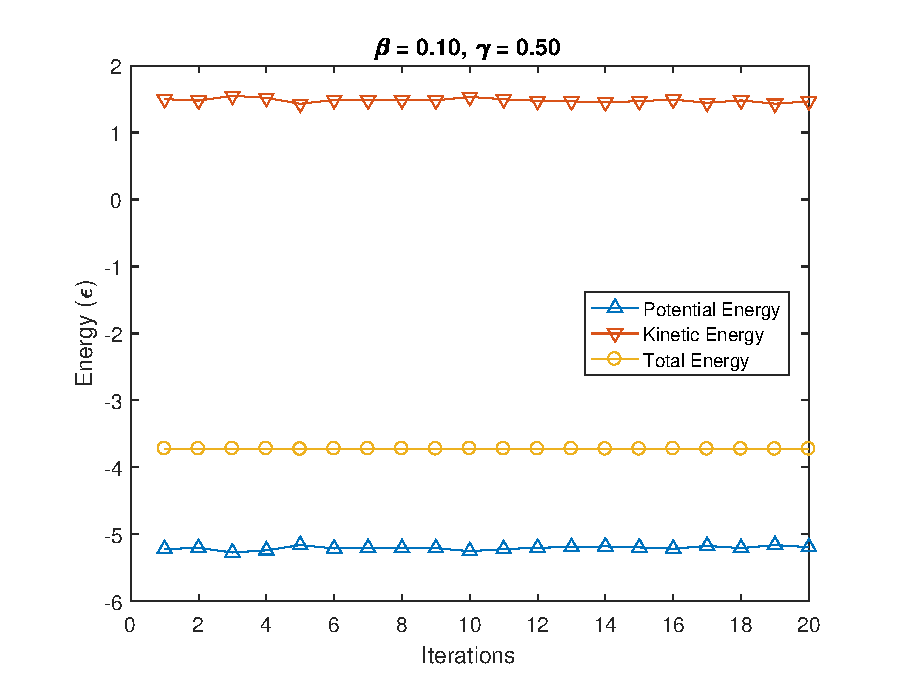
\includegraphics[width=0.5\textwidth]{energy_b0,10_g0,50.eps} &
    		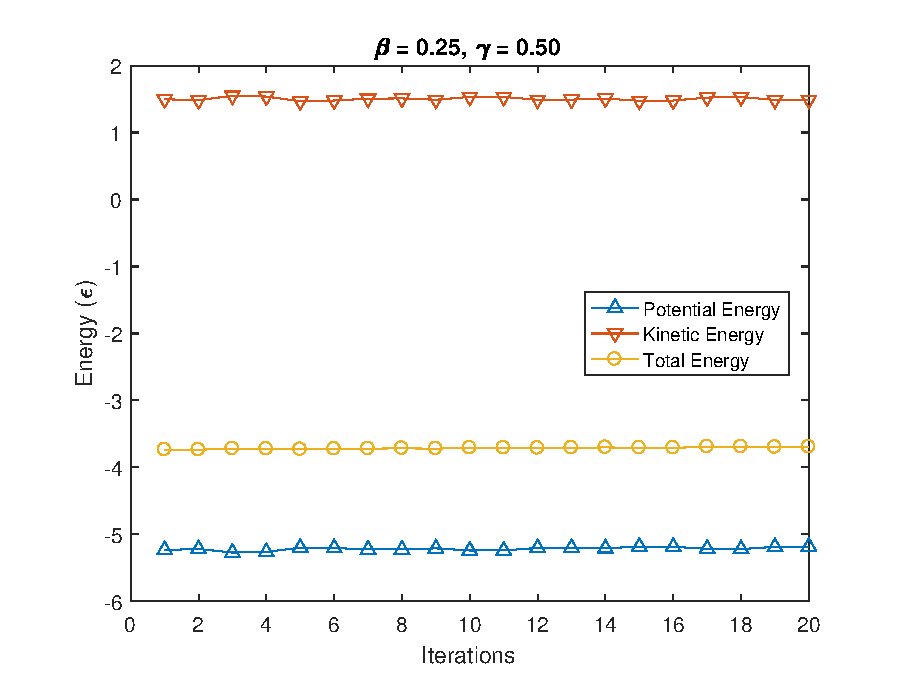
\includegraphics[width=0.5\textwidth]{energy_b0,25_g0,50.eps} \\
    		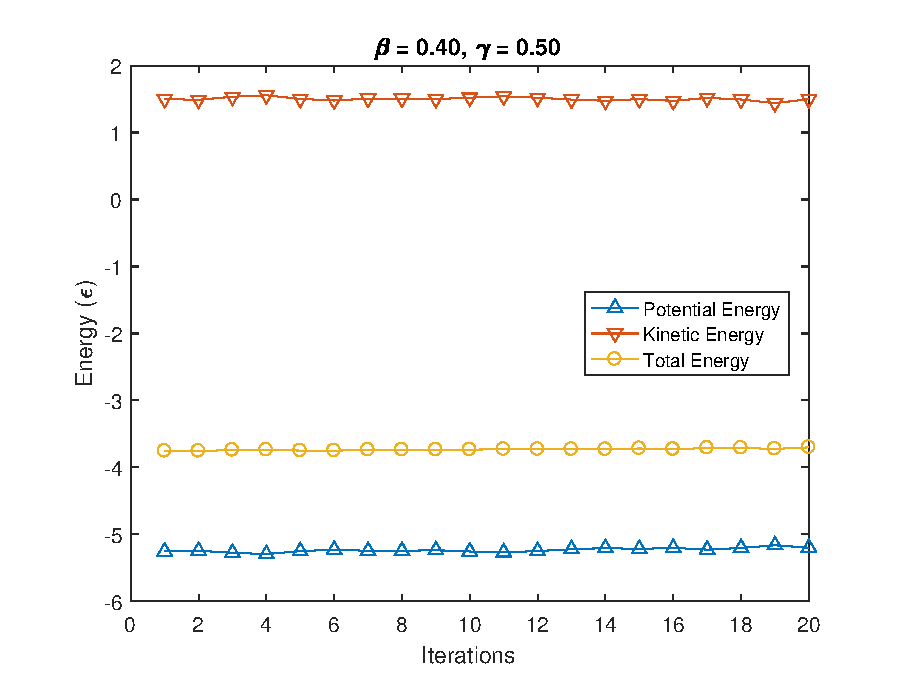
\includegraphics[width=0.5\textwidth]{energy_b0,40_g0,50.eps} &
    		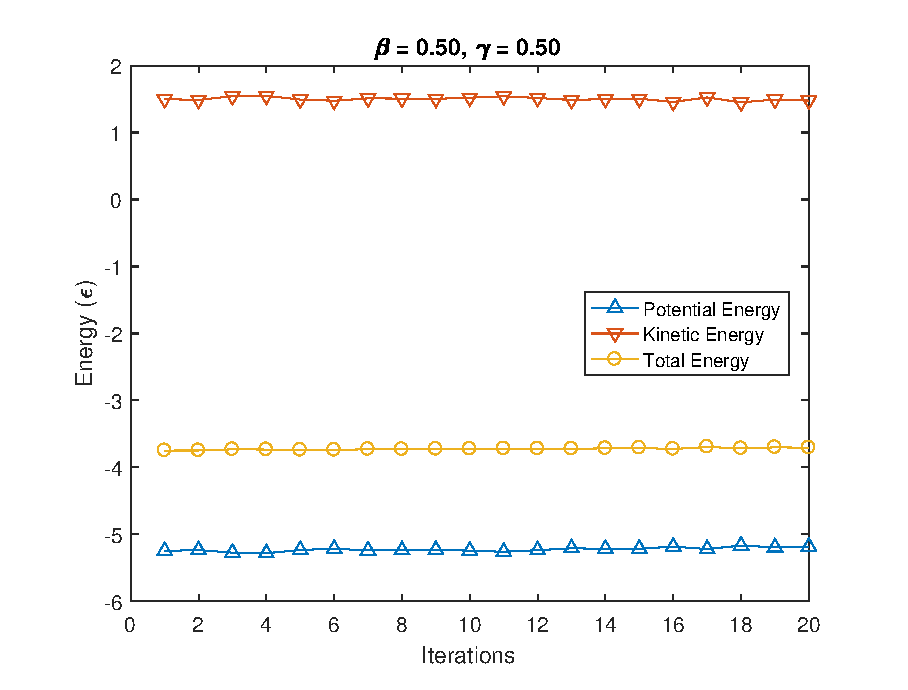
\includegraphics[width=0.5\textwidth]{energy_b0,50_g0,50.eps} \\
	\end{tabular}
  	\caption{Energy time series for implicit Newmark Beta methods with $\gamma = 0.50$}
	\label{fig:energy_time_series_gamma_0,50_implicit_beta}
\end{figure} 

Figure~\ref{fig:energy_time_series_gamma_0,50_implicit_beta}, however, brings bad news. We see that the graphs depict energy being conserved for every value of $\beta$ tested. This contradicts the quote above, which states that the implicit Newmark Beta methods are not designed to preserve energy. This highlights that the simplification in our initial configuration could have actually caused problems such that the system may not have been properly equilibrated before it was sampled. It is untenable to run simulations with the initial configurations defined in Table~\ref{tbl:initial_configuration_simulation} for all permissible values of $\beta$.
Thus, we need to consider a way to reduce the possible candidates that we review. Looking at literature, the trapezoidal rule $\left(\beta = 0, \gamma = \frac{1}{2}\right)$ is mentioned quite often - with \cite{DoyenErnPiperno2011} and \cite{Krenk} showing that the trapezoidal equation convserves energy balance. Figure~\ref{} shows the results of running the simulation with unmodified initial configurations with the Trapezoidal Rule, and it seems to corroborate the observation that the Trapezoidal Rule will conserve total energy. How does this observation then not contradict the results of \cite{SimoTarnowWong1992}? This is because the authors of  \cite{SimoTarnowWong1992} were referring to case of an arbitrary nonlinear Hamiltonian system - that ``textit{For an arbitrary nonlinear Hamiltonian system, the central difference method is the only symplectic scheme within the family of Newmark algorithms.}''

Before concluding that the Trapezoidal Rule conserves energy for the Hamiltonian in question, we need to confirm that the observations are not similar to those in Figure~\ref{fig:energy_time_series_gamma_0,50_implicit_beta}. As the last trial took almost 2200 seconds to compute, we cannot use for this technique. Instead, we first equilibrate the system using the Velocity Verlet algorithm, and provide the equilibrated state as the initial state to the methods being investigated. As the Velocity Verlet algorithm conserves total energy, the total energy of the state being provided will not be too different from the total energy of the initial state. So, we are using the unmodified initial configurations, except that $N_{e} = 0$ for the implicit Newmark Beta method. Figures~\ref{fig:energy_time_series_beta_0,10_gamma_0,50_long} and \ref{fig:energy_time_series_beta_0,40_gamma_0,50_long} show the results of the simulation on two different values of $\beta$ - 0.10 and 0.40. Both these figures depict total energy being conserved over the long run. In fact, the behaviour of both these systems is extremely similar to the behaviour of the system with $\beta = 0.25$, which raises the question - does $\beta$ have no effect on the solutions of the system? However, the problem can be related to our handling of $\beta$ as well - using Newton-Raphson Iterations multiplied $\beta$ by $h^{2}$ and $\vec{J}_{\vec{a}_{i+1}}$ - two very small in magnitude. This would have masked the contributions of $\beta$ to the solutions of the system.

Nevertheless, we cannot state with certainty whether the Trapezium Rule - or any other implicit Newmark Beta rules - conserve total energy. We can, however, state that the Velocity Verlet algorithm is symplectic, and hence, conserves the total energy in the system. 
\begin{figure}[H]
\centering
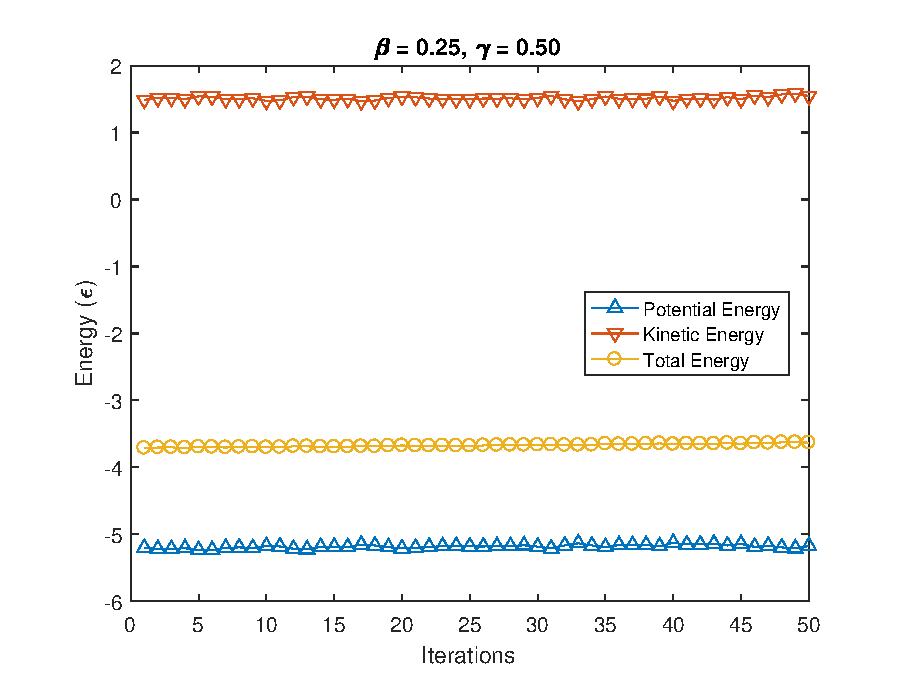
\includegraphics[scale=0.65]{energy_b0,25_g0,50_long.eps}
\caption{Energy time series for Newmark Beta methods with $\beta = 0.25$  and $\gamma = 0.50$ under unmodified initial configurations}
\label{fig:energy_time_series_beta_0,25_gamma_0,50_long}
\end{figure}

\begin{figure}[H]
\centering
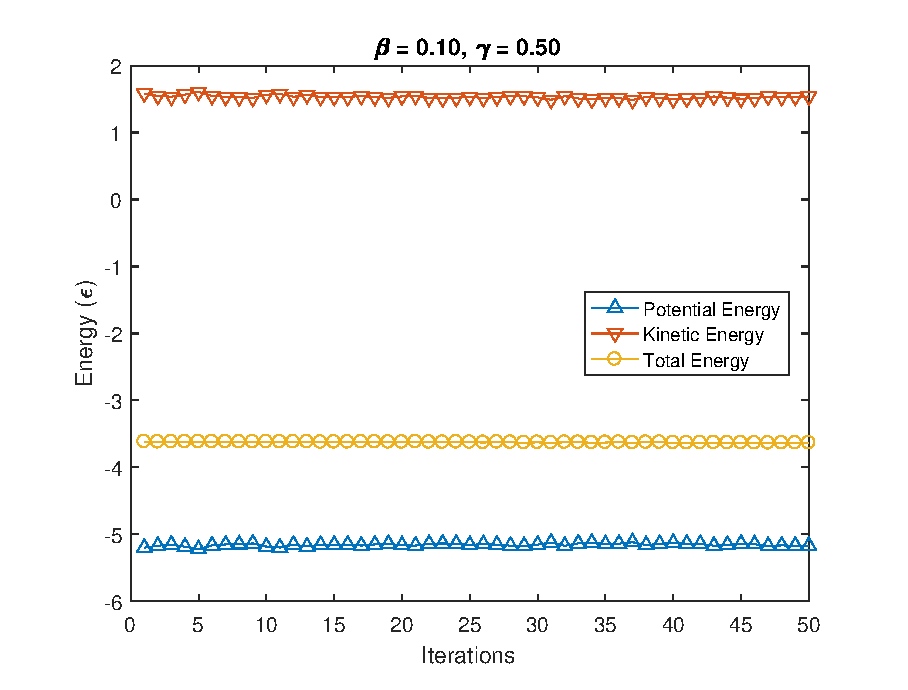
\includegraphics[scale=0.65]{energy_b0,10_g0,50_long.eps}
\caption{Energy time series for Newmark Beta methods with $\beta = 0.10$  and $\gamma = 0.50$ under unmodified initial configurations}
\label{fig:energy_time_series_beta_0,10_gamma_0,50_long}
\end{figure}

\begin{figure}[H]
\centering
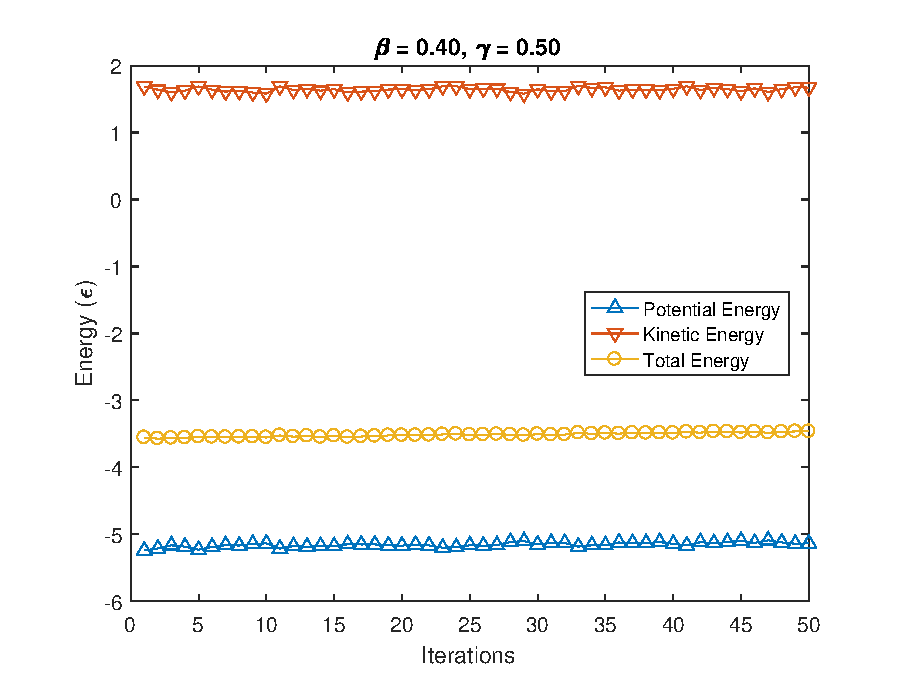
\includegraphics[scale=0.65]{energy_b0,40_g0,50_long.eps}
\caption{Energy time series for Newmark Beta methods with $\beta = 0.40$  and $\gamma = 0.50$ under unmodified initial configurations}
\label{fig:energy_time_series_beta_0,40_gamma_0,50_long}
\end{figure}
\centering

\end{document}
